% TEMPLATE for Usenix papers, specifically to meet requirements of
%  USENIX '05
% originally a template for producing IEEE-format articles using LaTeX.
%   written by Matthew Ward, CS Department, Worcester Polytechnic Institute.
% adapted by David Beazley for his excellent SWIG paper in Proceedings,
%   Tcl 96
% turned into a smartass generic template by De Clarke, with thanks to
%   both the above pioneers
% use at your own risk.  Complaints to /dev/null.
% make it two column with no page numbering, default is 10 point

% Munged by Fred Douglis <douglis@research.att.com> 10/97 to separate
% the .sty file from the LaTeX source template, so that people can
% more easily include the .sty file into an existing document.  Also
% changed to more closely follow the style guidelines as represented
% by the Word sample file. 

% Note that since 2010, USENIX does not require endnotes. If you want
% foot of page notes, don't include the endnotes package in the 
% usepackage command, below.

% This version uses the latex2e styles, not the very ancient 2.09 stuff.
\documentclass[letterpaper,twocolumn,10pt]{article}
\usepackage{usenix,epsfig,endnotes,graphicx}
\usepackage{epstopdf}
% \DeclareGraphicsExtensions{.eps}

\begin{document}

%don't want date printed
\date{}

%make title bold and 14 pt font (Latex default is non-bold, 16 pt)

\title{\Large \bf BugBox : A Vulnerability Corpus for PHP Web Applications}


%for single author (just remove % characters)
\author{
{\rm Kent Wills}\\
Computer Science Department\\University of Maryland
\and
{\rm Gary Nilson}\\
Computer Science Department\\University of Maryland
% copy the following lines to add more authors
% \and
% {\rm Name}\\
%Name Institution
} % end author

\maketitle

% Use the following at camera-ready time to suppress page numbers.
% Comment it out when you first submit the paper for review.
\thispagestyle{empty}

\subsection*{Abstract}

This paper covers the motivation and architecture behind BugBox, an open-source collection and management framework for PHP web application vulnerabilities. It is recognized that obtaining an adequate vulnerability dataset is a major hurdle in empirical vulnerability research. Many studies suffer from using vulnerability data-sets that are too small and often not made publicly available [ref]. The purpose of BugBox is to fill this void, and in doing so encourage the quality and repeatability of results. The goal is to collect a large number of vulnerabilities accross many applications, and make data available to the larger community. Example uses of BugBox include testing vulnerability indicators and metrics, developing vulnerability definition representations, testing intrusion detection systems, or creating demonstrations for training purposes. 

\section{Introduction}latex verbatim indentation
(i.e. Introduction and Motivation)
[what is a corpus?
 what is empirical vulnerability research?
 what should a corpus contain?
 what cool things can BugBox do?]

As researchers we can gain knowledge about vulnerable code through analyzing previously run exploits.  Understanding why code is vulnerable can lead to automated techniques in preventing future vulnerabilities.  In order to conduct this analysis, we must build a corpus.  

Building a corpus is not usually the main focus in conducting research.  Typically researchers want to develop their corpus quickly so that they can move on to the more important work, research. 
Understanding the labor involved in developing a corpus that suits the needs of a researcher, we propose an elegant [GJN!] framework using current tools in order to automate data collection in a simple and scalable way.  
Furthermore, we propose to increase our vulnerability corpus through a community approach and share our framework so that researchers will have a reference implementation.\endnote{Remember to use endnotes, not footnotes!}


A useful corpus is one that has a diverse selection of applications in addition to a large sampling of vulnerabilities. However, quanitity is not the only important requirement. Special consideration is made so that all relavant details of a vulnerability are available to the researcher. For a given application, the corpus includes the software in which a vulnerability exists, the configuration of the software in it's vulnerable state, exploit code that will trigger the security breach, and any other relavant attributes.\\
Through the use of abstraction and encapsulation, the management of application, environment, and exploitation can be streamlined. 

[Diversity, Quantity, Automation, Ease-of-use, Collaboration]

Why PHP?
At it's core, the vulnerability engine is driven by Python. Python's modules and Packages form the organizational basis for the project, with exploits, applicaitons, and application plugins having been abstracted out .... blah blah
Why Python?

Exploit Sources:\\
 \begin{tabular} { l }
   $\bullet$ Vulnerability Databases [Inj, NVD, OSVDB, exp]\\
   $\bullet$ Vulnerability Frameworks (Metasploit, etc...)\\
 \end{tabular}
\\

Key qualities:\\
 \begin{tabular}{ l }
   $\bullet$ Quantity of vunlerabilities\\
   $\bullet$ Diversity of applications\\
   $\bullet$ Automation of trace collection\\
   $\bullet$ Collaboration from other researchers\\
   $\bullet$ Ease of exploit implementation\\

 \end{tabular}
\\


\subsection{Empirical Vulnerability Research}


A key question in empirical vulnerability research is how to determine which functionality, or piece of code creates a vulnerable condition in a program. In studying this problem, sometimes referred to as \emph{vulnerability localization}, it is necessary to have a large quantity of structured data on which one can formulate and test hypotheses. Since potential approaches include vulnerability definitions based both static and dynamic analysis of the software, it is important that the corpus include both the vulnerable program's code, and some way to perform analysis as the system is compromized.\\


[many things with with references go here]


. In any case, an ideal vulnerability corpus would make it easy to explore each of these domains. 

Demonstrate that BugBox ....

Should be x, should be y, and should be z.

 Predicting which metrics  

The design a practical system for managing a database of exploits, along with their target environments. 

Code inspection
Trace-based vulnerability definitions
System taint analysis

Selenium ... 


``Vulnerability localization''

Characteristics:\\
 \begin{tabular} { l }
   -Collecting Vulnerable Application source code\\
   -Collecting vulnerability details\\
     a) line-based\\
     b) run-based\\
      i. trace-based\\
 \end{tabular}\\



\section{Framework}

Our framework has three main components: Web Application Store, Testing Environment, and Testing Scripts. 
These elements are reside in the following folders: backups, exploits, live systems, packages, and scripts. [GJN REFER TO DIAGRAM]


% you can also use the wonderful epsfig package...
%{\special{psfile = system_diagram.ps hscale = 50 vscale = 50}}
\begin{figure}[t]

\begin{center}
\begin{picture}(300,150)(0,15) %(0,200)
\put(0,0){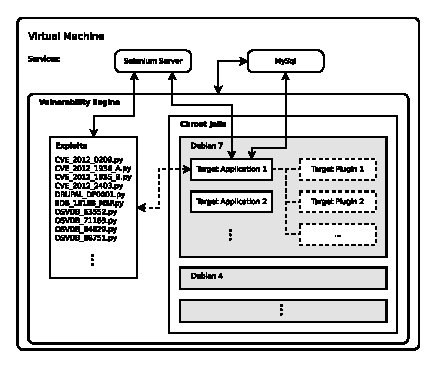
\includegraphics[scale=1.17]{system_diagram.eps}}
\end{picture}\\
\end{center}
\caption{System Diagram}
\end{figure}

\subsection{Vulnerability Engine}

Currently the framework provides support for PHP Web Applications.  We are restricted to web applications because of the use of selenium scripts in our corpus. [GJN ADD NOTES FROM JEFF's PAPER ON THIS]  
While we cannot alter the type of application, we do see future support for other languages [GJN YES].  
We are currently tied to PHP because we use XDebug as our trace collector [GJN NO].  
Our framework could be extended to any language that has a tool that trace the execution of the web application.  
All applications are currently package in a zip folder and are labeled by application name and version number. [GJN packaged as python modules that ]  

Architecture:

  The Host Machine
    (Why VM?).. future decision
    Selenium Server
    Mysql
  Vulnerability Engine
    Chroot Jails
    Application Modules
    The Exploit


\subsection{Environment}

Figure 1 illustrates general structure of the corpus environment. The system was designed to be modular. Being able to interchange every component from the application plugin level, all the way up to the engine, 

\subsubsection{Environment Setup}

The corpus contains a main engine, written in python, to load a web application, gather traces, run exploits, and cleanup.  We provide an engine to abstract away the details of the setup process so that contributors can focus on creating new exploit scripts.  This separation accomplished two tasks, it makes developing for the corpus more approachable for programmers that want to contribute and provides a robust framework that can provide more of a challenge to seasoned programmers.

\subsubsection{Chroot Jails}


We use a virtual jail, the linux chroot environment.  Staging the application in the chroot environment provides locality, reproducibility, and stability.  

{\bf The web application remains local}.  Many applications, such as wordpress, have a MYSQL backend.  If we were to host the application on a different server or VM we would have to ensure that the MYSQL database is properly setup each time.  With the chroot environment, the process is simplified, we keep a MYSQL database outside of the CHROOT Jail in order to facilitate MYSQL access.  

{\bf Current tests are independent from future tests}.  We load a clean application into the chroot jail every time we wish to run a new test.  This ensures that there is no corruption of the original Web Application and provides reproducible results when testing.

{\bf The web application cannot contaminate our testing environment}.  If a web application crashes due to the malicious script, we can ensure that it does not crash our corpus environment, worst case the chroot is corrupted, and we can ensure that the crash cannot have un-intended side effects in our testing environment.  

\subsubsection{Target Module}

Submodules: (package corpus)\\
 \begin{tabular}{ l }
   $\bullet$ corpus.Targets\\
   $\bullet$ corpus.Engine\\
   $\bullet$ corpus.Exploit\\
   $\bullet$ corpus.SeleniumDriver\\
 \end{tabular}\\

 \begin{description}
   \item[Targets] contains a module for every target application.
   \item[Engine] drives the environment setup, tear-down, and exploit process.
   \item[Exploit] a superclass for each exploit in the corpus.
   \item[SeleniumDriver] a wrapper class for the Slenium's Firefox web driver.
 \end{description}

\subsection{Exploit}

Management actions, recording commands
attributes, 

\subsubsection{As a Standalone Application}

Each exploit is defined in it's own python file as a module. In Python, modules can either be imported from other modules, or executed directly from the command-line. The exploits written for BugBox take advantage of this property to give the researcher the option of writing scripts to do work on a set of exploits, or to invoke one exploit at a time. When run from the command-line, the supplied arguments are passed directly to the vulnerability engine, which supports the options shown below: 


{\tt \footnotesize
\begin{verbatim}
Usage: python OSVDB_89960.py [options]
Options:
    start:          Start exploit instance
    stop:           Stop exploit instance
    exploit:        Run the exploit
    check:          Check if the corresponding 
                    environment is running
    xdebug_on:      Turn on xdebug autotrace
    xdebug_off:     Turn off and collect 
                    xdebug autotrace
\end{verbatim}}

\subsubsection{As a Python Module}



corpus.Query interface


\subsubsection{Selenium Scripts}

We aim to gather code that is vulnerable.  We drastically can reduce the amount of computation needed by reducing the code size that needs to be analyzed through the use of past, found exploits.  

In order to better isolate vulnerable code, we create a selenium script in Python, replicating actions a user would take in performing an exploit on a web application.  While the script is running, we can have XDebug monitor the execution and output the final execution trace for the selenium script execution.  We can see future additions to this by turning XDebug on and off through cookie manipulation while the script is running, furthermore reducing the size of the vulnerable code.

By setting up the application loader engine, we are able to create concise python selenium scripts for data collection.  The following code shows how easy it is to run an automated exploit:

Pros:
-Ease of use
-Uses browser's javascript engine
-Good for visualization

Cons:
-Not a necessary dependancy, urrllib+cookielib would suffice
-requires SeleniumServer to run as a service on the host system
P

{\tt \footnotesize
\begin{verbatim}

payload = "XSS PAYLOAD"

driver = self.create_selenium_driver()

driver.get("http://localhost/wordpress/?p=1")

%Selenium Actions preceded by
% driver.find_element_by_id
("author").clear()
("author").send_keys("selenium script")
("email").clear()
("email").send_keys("selenium@python.org")
("url").clear()
("url").send_keys("www.python.org")
("comment").clear()
("comment").send_keys(payload)
("submit").click()

\end{verbatim}}


\subsection{File Structure}

The file structure mimics the modularity of our corpus.  Currently we store backups of the Web Applications in the {\tt/backups} directory and the actual applications in the {\tt/packages} directory.  We store a separate backup in order to verify that the selenium scripts did not modify the Web Application in any way.  If the Web Application is corrupt, then we simply copy the web application from the backup folder to the package folder.  

Currently as simple incremental backup system is used to ensure that each chroot jail remains un-tainted. Periodically, an original instance of a chroot system will overwrite the 

Future implementations will store only the md5 hash of the program on the corpus server and the backups on an external server.  This will allow for a quick comparison followed by a remote copy if necessary.  This separation will ensure that backups will never be corrupted through use of the corpus.  

All the exploits that are available are located under the {\tt /scripts} folder.  While script is referenced as Selenium Script throughout the document, here scripts also include services such as: deploying the web application in the chroot jail, starting the trace collection, and running the script. All mounted chroot environments reside in {\tt /live\_systems}. 
\\\\
{\bf insert file system diagram}



\section{Scalability}
In order to create a system that can handle a growing amount of vulnerabilities that are independent from one another, we represent an exploit on an application through  Selenium scripts, as noted in the Framework section.  Selenium scripts allow us to perform operations on web applications without fear of working in an un-intended, compromised environment. 

\section{Usability}
By providing a corpus that explicitly logs the steps taken in accumulating the log files, we have more flexibility.  This flexibility can be seen with the following example:  
\\\\
{\tt Jon is told by his advisor that he needs to collect more trace data in order to get a proper sample size for his research.  John quickly creates a selenium script for the exploit he wants to collect and shows the advisor his results.  The advisor was generally happy with the trace data that he collected, but instead wanted him to do a slight modification to the exploit.  If Jon did not have the selenium script at hand, he would have to duplicate all of the work previously done.  Since he does have the script on hand, he can quickly make a change to the script and re-run in seconds versus hours.}
\\\\
While the above process is only shown in one iteration, most students know that this is not the case.  One hour of work can turn into a whole week of work without the proper framework in place.  The above situation also shows that the selenium script can be discussed with the professor to show validity of the data and provide talking points for how the exploit was applied.


\section{Related Work}

Some embedded literal typset code might 
look like the following :

{\tt \small
\begin{verbatim}
int wrap_fact(ClientData clientData,
              Tcl_Interp *interp,
              int argc, char *argv[]) {
    int result;
    int arg0;
    if (argc != 2) {
        interp->result = "wrong # args";
        return TCL_ERROR;
    }
    arg0 = atoi(argv[1]);
    result = fact(arg0);
    sprintf(interp->result,"%d",result);
    return TCL_OK;
}
\end{verbatim}
}

Now we're going to cite somebody.  Watch for the cite tag.
Here it comes~\cite{Chaum1981,Diffie1976}.  The tilde character (\~{})
in the source means a non-breaking space.  This way, your reference will
always be attached to the word that preceded it, instead of going to the
next line.

\section{Future Development}
 \begin{description}
   \item[Distribution]
     Virtual machine v.s. debian package. Pre-built chroot jails v.s. build scripts.
   \item[Services]
     Why run Selenium/Mysql in VM vs a chroot jail?\\
   \item[Isolating attack event]
 (with xdebug manually/cookies/etc...)   
   \item[Payload standardization]
For each exploit currently in the corpus, there is no standard for the payload used in the attack. Since many studies may be sensitive to the payload type and encoding, it makes sense to provide the researcher with fine-grained control over this property. The Metasploit Framework has a very robust system for managing exploits along with their payloads and encodings, and can be a model for implementing this.
 \end{description}


\section{Conclusion}

Conclusion

\section{Availability}

[Available as a 10 GB virtual machine and as a standalone debian package]

\begin{center}
{\tt ftp://ftp.site.dom/pub/myname/Wonderful}\\
{\tt git://bugbox.github.com/blahblah}\\
\end{center}

Also, it's even greater when you can write that information is also 
available on the Wonderful homepage at 

\begin{center}
{\tt http://www.vulnerabilitywiki.com/\~{}myname/SWIG}
\end{center}

Now we get serious and fill in those references.  Remember you will
have to run latex twice on the document in order to resolve those
cite tags you met earlier.  This is where they get resolved.
We've preserved some real ones in addition to the template-speak.
After the bibliography you are DONE.

{\footnotesize \bibliographystyle{acm}
\bibliography{../common/bibliography}}


\theendnotes

\end{document}







